%% ----------------------------------------------------------------
%% Report.tex
%% ---------------------------------------------------------------- 
\documentclass{ecsreport}      % Use the Report Style
\graphicspath{{../Figures/}}   % Location of your graphics files
\usepackage{natbib}            % Use Natbib style for the refs.
\hypersetup{colorlinks=true}   % Set to false for black/white printing
%% ----------------------------------------------------------------
%% Definitions.tex
%% ---------------------------------------------------------------- 
\newcommand{\BibTeX}{{\rm B\kern-.05em{\sc i\kern-.025em b}\kern-.08em T\kern-.1667em\lower.7ex\hbox{E}\kern-.125emX}}
\def\myrotate{\ifodd\c@page\else-\fi 90}
%% People
\newcounter{address}
\setcounter{address}{1}
\renewcommand{\theaddress}{\textsuperscript{\fnsymbol{address}}}
\newcommand{\address}[1]{\refstepcounter{address}\theaddress#1\\}
\newcommand{\Name}[3]{\texorpdfstring{\href{mailto:#3}{#2}#1}{#2}\xspace}
\newcommand{\SteveRGunn}[1]{\Name{#1}{Steve R. Gunn}{S.R.Gunn@ecs.soton.ac.uk}}

%% Dingbats
\newcommand{\tick}{\ding{51}}
\newcommand{\cross}{\ding{55}}

%% Calculus
\newcommand{\pd}[2]{\ensuremath{\frac{\partial #1}{\partial #2}}\xspace}
\newcommand{\fd}[2]{\ensuremath{\frac{d #1}{d #2}}\xspace}
\newcommand{\dint}{\ensuremath{\int\!\!\!\int}\xspace}
\newcommand{\tint}{\ensuremath{\int\!\!\!\int\!\!\!\int}\xspace}

%% Math Sets
\newcommand{\Q}[1]{\ensuremath{\mathbb{#1}}\xspace}
\newcommand{\R}{\Q{R}}

%% Matrix, Vector
\newcommand{\V}[1]{\ensuremath{\boldsymbol{#1}}\xspace}
\newcommand{\M}[1]{\ensuremath{\boldsymbol{#1}}\xspace}
\newcommand{\0}{\V{0}}
\newcommand{\1}{\V{1}}
\newcommand{\I}{\M{I}}

%% Math Functions
\newcommand{\F}[1]{\ensuremath{\mathrm{#1}}\xspace}
\newcommand{\sgn}{\F{sgn}}
\newcommand{\tr}{\F{trace}}
\newcommand{\diag}{\F{diag}}

%% Math Names
\newcommand{\N}[1]{\ensuremath{\mathit{#1}}\xspace}

%% Data
\newcommand{\mc}[1]{\ensuremath{\mathcal{#1}}\xspace}
\newcommand{\Hyp}{\mc{H}}
\newcommand{\D}{\mc{D}}

%% Kernel
\newcommand{\K}{\M{K}}
\newcommand{\eins}{\texorpdfstring{\ensuremath{\epsilon}}{\textepsilon}-insensitive\xspace}
\newcommand{\e}{\ensuremath{\epsilon}\xspace}
\newcommand{\Bxi}{\ensuremath{\boldsymbol{\xi}}\xspace}
\newcommand{\Kanova}{\ensuremath{\mathit{K_{ANOVA}}}\xspace}
\newcommand{\Kspline}{\ensuremath{\mathit{K_{spline}}}\xspace}

%% Bayesian
\newcommand{\MP}{\ensuremath{\mathit{{\scriptscriptstyle \hspace{-1.5pt}M\hspace{-1.5pt}P}}}\xspace}
\newcommand{\ML}{\ensuremath{\mathit{{\scriptscriptstyle \hspace{-1.5pt}M\hspace{-1.5pt}L}}}\xspace}
\newcommand{\Qw}{\ensuremath{Q_{\w}(\w)}\xspace}
\newcommand{\Qa}{\ensuremath{Q_{\Ba}(\Ba)}\xspace}
\newcommand{\Qb}{\ensuremath{Q_{\beta}(\beta)}\xspace}
\newcommand{\wMPab}{\ensuremath{\w_{\MP|\bar {\Ba},\bar \beta}}\xspace}
\newcommand{\wMP}{\ensuremath{\w_{\MP}}\xspace}
\newcommand{\yMP}{\ensuremath{y_{\MP}}\xspace}
\newcommand{\BaMP}{\ensuremath{\Ba_{\hspace{1pt}\MP}}\xspace}
\newcommand{\aMP}{\ensuremath{\alpha_{\hspace{1pt}\MP}}\xspace}
\newcommand{\bMP}{\ensuremath{\beta_{\hspace{1pt}\MP}}\xspace}
\newcommand{\Sab}{\ensuremath{\M{\Sigma}_{\bar \Ba,\bar \beta}}\xspace}
\newcommand{\Ba}{\ensuremath{\boldsymbol{\alpha}}\xspace}
\newcommand{\Bb}{\ensuremath{\boldsymbol{\beta}}\xspace}
\newcommand{\Bm}{\ensuremath{\boldsymbol{\mu}}\xspace}
\newcommand{\BL}{\ensuremath{\boldsymbol{\Lambda}}\xspace}
\newcommand{\BPhi}{\ensuremath{\boldsymbol{\Phi}}\xspace}
\newcommand{\SMP}{\ensuremath{\M{\Sigma}_{\MP}}\xspace}

\newcommand{\Pa}{\ensuremath{P(\alpha|\mathcal{H})}\xspace}
\newcommand{\Pb}{\ensuremath{P(\beta|\mathcal{H})}\xspace}
\newcommand{\Pab}{\ensuremath{P(\alpha,\beta|\mathcal{H})}\xspace}
\newcommand{\Pw}{\ensuremath{P(\w|\mathcal{H})}\xspace}
\newcommand{\PD}{\ensuremath{P(\D|\mathcal{H})}\xspace}
\newcommand{\PwIa}{\ensuremath{P(\w|\alpha,\mathcal{H})}\xspace}
\newcommand{\PDIwb}{\ensuremath{P(\D|\w,\beta,\mathcal{H})}\xspace}
\newcommand{\PDwab}{\ensuremath{P(\D,\w,\alpha,\beta|\mathcal{H})}\xspace}
\newcommand{\PDIw}{\ensuremath{P(\D|\w,\mathcal{H})}\xspace}
\newcommand{\PwID}{\ensuremath{P(\w|\D,\mathcal{H})}\xspace}
\newcommand{\PwabID}{\ensuremath{P(\w,\alpha,\beta|\D,\mathcal{H})}\xspace}

\newcommand{\PanH}{\ensuremath{P(\alpha)}\xspace}
\newcommand{\PbnH}{\ensuremath{P(\beta)}\xspace}
\newcommand{\PabnH}{\ensuremath{P(\alpha,\beta)}\xspace}
\newcommand{\PwnH}{\ensuremath{P(\w)}\xspace}
\newcommand{\PDnH}{\ensuremath{P(\D)}\xspace}
\newcommand{\PwIanH}{\ensuremath{P(\w|\alpha)}\xspace}
\newcommand{\PDIwbnH}{\ensuremath{P(\D|\w,\beta)}\xspace}
\newcommand{\PDwabnH}{\ensuremath{P(\D,\w,\Ba,\beta)}\xspace}
\newcommand{\PDIwnH}{\ensuremath{P(\D|\w)}\xspace}
\newcommand{\PwIDnH}{\ensuremath{P(\w|\D)}\xspace}
\newcommand{\PwabIDnH}{\ensuremath{P(\w,\alpha,\beta|\D)}\xspace}

\newcommand{\PDwBab}{\ensuremath{P(\D,\w,\Ba,\beta|\mathcal{H})}\xspace}
\newcommand{\PwIBa}{\ensuremath{P(\w|\Ba,\mathcal{H})}\xspace}
\newcommand{\PBab}{\ensuremath{P(\Ba,\beta|\mathcal{H})}\xspace}
\newcommand{\PwBabID}{\ensuremath{P(\w,\Ba,\beta|\D,\mathcal{H})}\xspace}

\newcommand{\PBanH}{\ensuremath{P(\Ba)}\xspace}
\newcommand{\PwIBanH}{\ensuremath{P(\w|\Ba)}\xspace}

%% Snakes
\newcommand{\Esnake}{\ensuremath{\mathit{E_{snake}}}\xspace}
\newcommand{\Eimage}{\ensuremath{\mathit{E_{image}}}\xspace}
\newcommand{\Econt}{\ensuremath{\mathit{E_{cont}}}\xspace}
\newcommand{\Ecurv}{\ensuremath{\mathit{E_{curv}}}\xspace}
\newcommand{\Eint}{\ensuremath{\mathit{E_{int}}}\xspace}
\newcommand{\Eext}{\ensuremath{\mathit{E_{ext}}}\xspace}
\newcommand{\Eterm}{\ensuremath{\mathit{E_{term}}}\xspace}
\newcommand{\Eline}{\ensuremath{\mathit{E_{line}}}\xspace}
\newcommand{\Eedge}{\ensuremath{\mathit{E_{edge}}}\xspace}
\newcommand{\Econ}{\ensuremath{\mathit{E_{con}}}\xspace}
\newcommand{\Eangle}{\ensuremath{\mathit{E_{angle}}}\xspace}
\newcommand{\Elshape}{\ensuremath{\mathit{E_{lshape}}}\xspace}
\newcommand{\Eedgedir}{\ensuremath{\mathit{E_{edgedir}}}\xspace}
\newcommand{\Emodel}{\ensuremath{\mathit{E_{model}}}\xspace}
\newcommand{\wte}{\ensuremath{\mathit{w_{term}}}\xspace}
\newcommand{\wli}{\ensuremath{\mathit{w_{line}}}\xspace}
\newcommand{\wed}{\ensuremath{\mathit{w_{edge}}}\xspace}
\newcommand{\wco}{\ensuremath{\mathit{w_{con}}}\xspace}

%% Environments
\newcounter{alg}
\newenvironment{algorithm}[1]
{
    \stepcounter{alg}
    \begin{table}[htb]
    \centering
    \begin{tabular}[t]{ll}
    \hline&\\
    \multicolumn{2}{l}{\bf Algorithm \arabic{alg}: #1}\\&\\
} {
    &\\
    \hline
    \end{tabular}
    \end{table}
}
%Code Styles
\lstset{basicstyle=\scriptsize\ttfamily,
        keepspaces=true,
        	numbers=left,
		numberstyle=\ttfamily\tiny,
		numberblanklines=false,
		stepnumber=1,
		numbersep=12pt,
		backgroundcolor=\color{black!2},
		showspaces=false,       
		showstringspaces=false,       
		showtabs=false,         
		frame=lrtb,
		rulecolor=\color{black!40}, 
		tabsize=4,
		captionpos=t,
		breaklines=true,
		breakatwhitespace=false,
		framesep=8pt,
		framerule=1pt,
		xleftmargin=9pt,
		xrightmargin=9pt,
		title=\lstname}
\lstdefinestyle{matlab} {
        language=Matlab,
        keywordstyle=\color{blue},
        commentstyle=\color[rgb]{0.13,0.55,0.13}\em,
        stringstyle=\color[rgb]{0.7,0,0} }
\lstdefinestyle{c} {
        language=C,
        keywordstyle=\color{blue},
        commentstyle=\color[rgb]{0,0.6,0},
        stringstyle=\color{red}
        }            % Include your abbreviations
%% ----------------------------------------------------------------
\begin{document}
\frontmatter
\title      {An Investigation into \dots}
\authors    {\texorpdfstring
             {\href{mailto:hl13g10@ecs.soton.ac.uk}{Henry S. Lovett}}
             {Henry S. Lovett}
            }
\addresses  {\groupname\\\deptname\\\univname}
\date       {\today}
\subject    {}
\keywords   {}
\maketitle
\begin{abstract}
This work is all about \dots
\end{abstract}
\tableofcontents
\listoffigures
\listoftables
\lstlistoflistings
\listofsymbols{ll}{$w$ & The weight vector}
\acknowledgements{Thanks to no one.}
\dedicatory{To \dots}
\mainmatter
%% ----------------------------------------------------------------
%% ----------------------------------------------------------------
%% Introduction.tex
%% ---------------------------------------------------------------- 
\chapter{Introduction} \label{Chapter:Introduction}
%The Introduction to my Report \dots

%The initial idea of the project was taken from Pirobot(\cite{Pirobot}).
%
%\inote{what it will do. Define everything. Use. Very general}
%General - mapping robots. 
%
%stereovision - uses etc.
%
%other similar projects
%
%why mine is important 

%\inote{Talk about what I set out to do, include some definitions etc. }
%\inote{What I ended up doing}
%\inote{The uses of my robot.} 

The original idea for the project was a stereoscopic mapping robot, similar to \cite{Pirobot}. This would autonomously search an area and return an occupancy map \citep{thrun2003learning}. The original project brief can be seen in Appendix \ref{Chapter:Appendix:Brief}. However, due to time constraints, the image processing aspects remain prototyped in MATLAB, but not implemented in C. The end robot is able to capture stereo image pairs, move with reasonable accuracy and compute Fourier Transforms. The robot can run a predefined set of commands automatically or act as a shell terminal.

Stereoscopy in computer vision is the ability to calculate the locations and depths using images from two or more cameras, which are used to triangulate and estimate distances \citep{Saxena:DepthEstimation}. By using two cameras on the same plane, separated by a set horizontal distance, the depth of the observed scene can be perceived by the system.

Stereo vision is a small section of computer vision which is widely used in many applications. Microsoft's Xbox Kinect \citep{Microsoft:Kinect} uses stereo vision to locate a game player in order to use their movements to control the game. \cite{Mrovlje:Distance_Stereoscopic} used stereo vision to be able to locate the distance to a marker. 
\inote{Leap Motion?}

The stereo vision robot discussed in this report is a low cost alternative to other robots which use laser range finders or high quality cameras \citep{Se:MappingRobot}. The robot was mounted on the base seen in Figure \ref{fig:RobotBase} and used two OmniVision OV7670 cameras delivering QVGA format images.

The final robot could be used for a variety of applications. The robot can perceive depth of the captured area so can avoid obstacles and navigate. The robot could also be adapted to stream the camera data to a remote computer, and be controlled by a user to explore unknown and potentially hostile areas safely. 

\begin{figure}
\centering
\includegraphics[width=\textwidth - 2cm]{./Figures/RobotBase.jpg}
\caption{The base of the robot}
\label{fig:RobotBase}
\end{figure}

\section{Project Management}
%In order to reduce the risk within the project, all aspects of potential issues were looked at and are summarised in table \ref{tab:risk}. A Gantt chart of how time was planned to be spent can be seen in figure \ref{fig:Gantt}.  

%The project was designed in stages - first, gaining operation of all the basic sections; movement, image capturing, image detection algorithms etc. These were then be brought together once tested to create the final product. This meant functionality was obtained of the basic aspects before addressing more complex issues. 

The project set ambitious targets. All sections of the design that needed addressing are seen in Table \ref{table:sections}. The project was developed using a spiral model to achieve the design aspects, starting with the hardware and firmware which were developed concurrently. This was done to obtain basic functionality first before concentrating on more complex aspects. Higher level algorithms were also prototyped during initial hardware development. However, the software was inherently dependant on the hardware. Therefore the hardware aspect was given priority. 

A number of risks were present during the project. These were assessed and steps were taken to reduce the chance of occurring. These can be seen in Table \ref{tab:risk}. 

At the beginning of the project, the Gantt chart in Figure \ref{fig:Gantt:1} was made. This was then reviewed after the interim report hand-in and Figure \ref{fig:Gantt:2} was made for how time should be spent during the second half of the project. Figure \ref{fig:Gantt:3} shows how time was actually spent during the project. 

Figure \ref{fig:Gantt:3} shows that more time was spent on testing than originally anticipated. Individual sections also arose small errors that were time consuming to correct, causing the time allocated to be insufficient. The motor driving also required a large change when porting to the AT32, causing time to be spent developing this further. 

\begin{table}
\centering
\caption{Hardware and Software aspects of the design}
\label{table:sections}
\begin{tabular}{cc}\toprule
\textbf{Hardware} & \textbf{Software} \\ \toprule
Single Camera	&	Firmware \\ \midrule
Dual Camera		&	Matching Algorithms \\ \midrule
SD Card			&	Range Finding \\ \midrule
Motor System	&	Mapping  \\ \midrule
PCB Design		&	Searching \\ \midrule
PCB Test		&	Testing \\ \bottomrule
\end{tabular}
\end{table}

\begin{table}
\centering
\caption{A list of risks and the prevention steps taken to reduce their impact}
\label{tab:risk}
\begin{tabular}{p{6cm}p{2cm}p{6cm}}\toprule
\textbf{Risk}						&	\textbf{Severity}	&	\textbf{Prevention} \\ \toprule
Components not arriving on time	&	High		&	Order parts as early as possible \\ \midrule
Project not fulfilling specification				&	High		&	Develop in stages to obtain functionality in parts. Ensure enough time is allocated to the project.	\\\midrule
PCB Design is incorrect		&	Medium		&	Check the design carefully and get second opinion. \\\midrule
Failure of personal computer causing data loss & Low	& 	Keep back ups of all work on Devtrack Git repository and Dropbox.\\
\bottomrule
\end{tabular}
\end{table}


%% ----------------------------------------------------------------
%% Conclusions.tex
%% ---------------------------------------------------------------- 
\chapter{Conclusions and Further Work} \label{Chapter: Conclusions}
%\section{Conclusion}

%\inote{What I have accomplished}
This work has led to a tested device which is mobile and has the capability to perform stereoscopic image processing. The system has the following parts:

\begin{enumerate}
\item Motor driving
\item Stereoscopic Cameras
\item SD Card memory
\item SRAM
\item Image Processing
\end{enumerate} 

The motor system is a simple, cheap method to move distances with reasonable accuracy. A better controller would allow variable speed and speed matching between motors. The system was shown to work to $4.5\%$ accuracy over a $300mm$ distance.

A full image can be read from a camera and stored on an SD card in a FAT32 file system. This gives the ability of removable memory that can be viewed on a computer to see any internal logs. Images are stored in QVGA format (320 by 240 pixels) as a bitmap image. 

An additional 4MB of SRAM memory is available to use on the robot allowing for large data arrays of the images to be kept in fast access RAM. The RAM is direct memory accessed so operation is almost seamless from internal memory.

Multiple comparison algorithms have been investigated and compared using the same test images. It was clear that, although at a necessity of more computations, the normalised cross correlation is the best with regard to overall reliability. 

The Fourier transform was also investigated and implemented. The system allows for a $2 \times 2$ array of a square image with dimensions of $2^{2n}\; $ where $n \in \mathbb{N}$ and is limited by RAM space and time. The transform is speed optimised and in tests proved to be fairly accurate. 

Range finding equations were then derived, which use the characteristics of the camera and the separation distance between them. %They have also been tested using MATLAB and images that have been rendered where all the distances are known and exact.

All aspects implemented on the robot have been shown to be functional. A faster processor would have been a good idea to use for image processing, but this could have developed other problems with the PCB. The Raspberry Pi or Steve Gunn's \textit{`L'Imperatrice'}, which both run a Linux operating system, would have been a good choice to remove the need for as much hardware design and existing image processing libraries could have been utilised to gain more functionality in the time. 

Though the robots original application wasn't achieved, the end device is a base for a stereoscopic application. The system is a tested platform for future applications to be implemented on and additions can be made using the spare pins and bus connections on the PCB headers. 

The system could be used in future projects to develop more functionality. Wireless communications could be added to the system to allow a connection to the computer and search algorithms can be implemented alongside distance calculations to make the robot aware of its surroundings. 
%\inote{What could be changed to make it better}
%\inote{Suggestions for further work}
\appendix
%% ----------------------------------------------------------------
%% AppendixA.tex Circuit Diagrams
%% ---------------------------------------------------------------- 
\chapter{Circuit Diagrams} \label{Chapter:AppendixA:CircuitDiagrams}
%\section{OV7670 Breakout Board Schematic}
\begin{figure}[ht!]
\centering
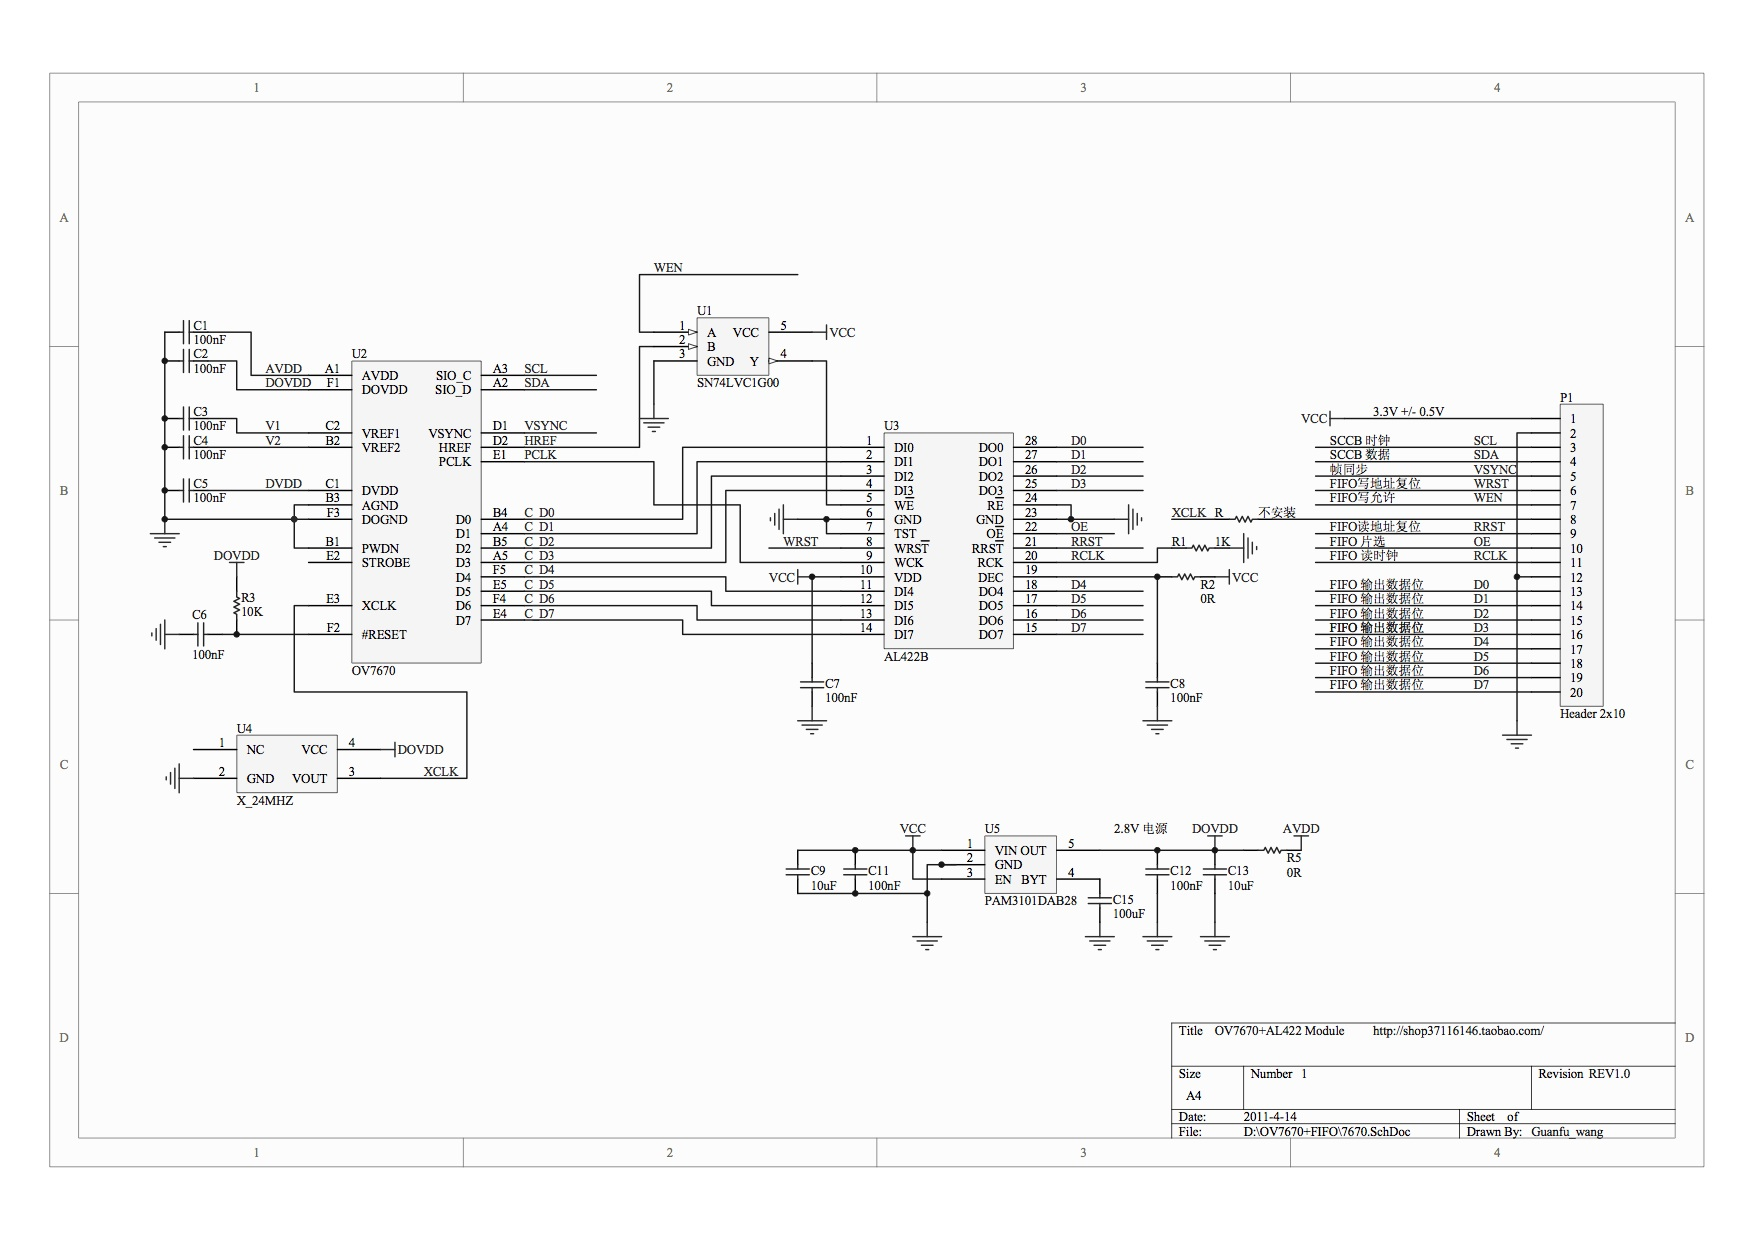
\includegraphics[angle=90,width=\textwidth,height=\textheight-10cm,keepaspectratio]{Figures/OV7670_Schematic.jpg} 
\caption{The circuit diagram for the OV7670 breakout board}
\label{OV7670_Schematic}

\end{figure}

%\section{Il Matto and Dual Camera Schematic}
\begin{figure}[ht!]
\centering
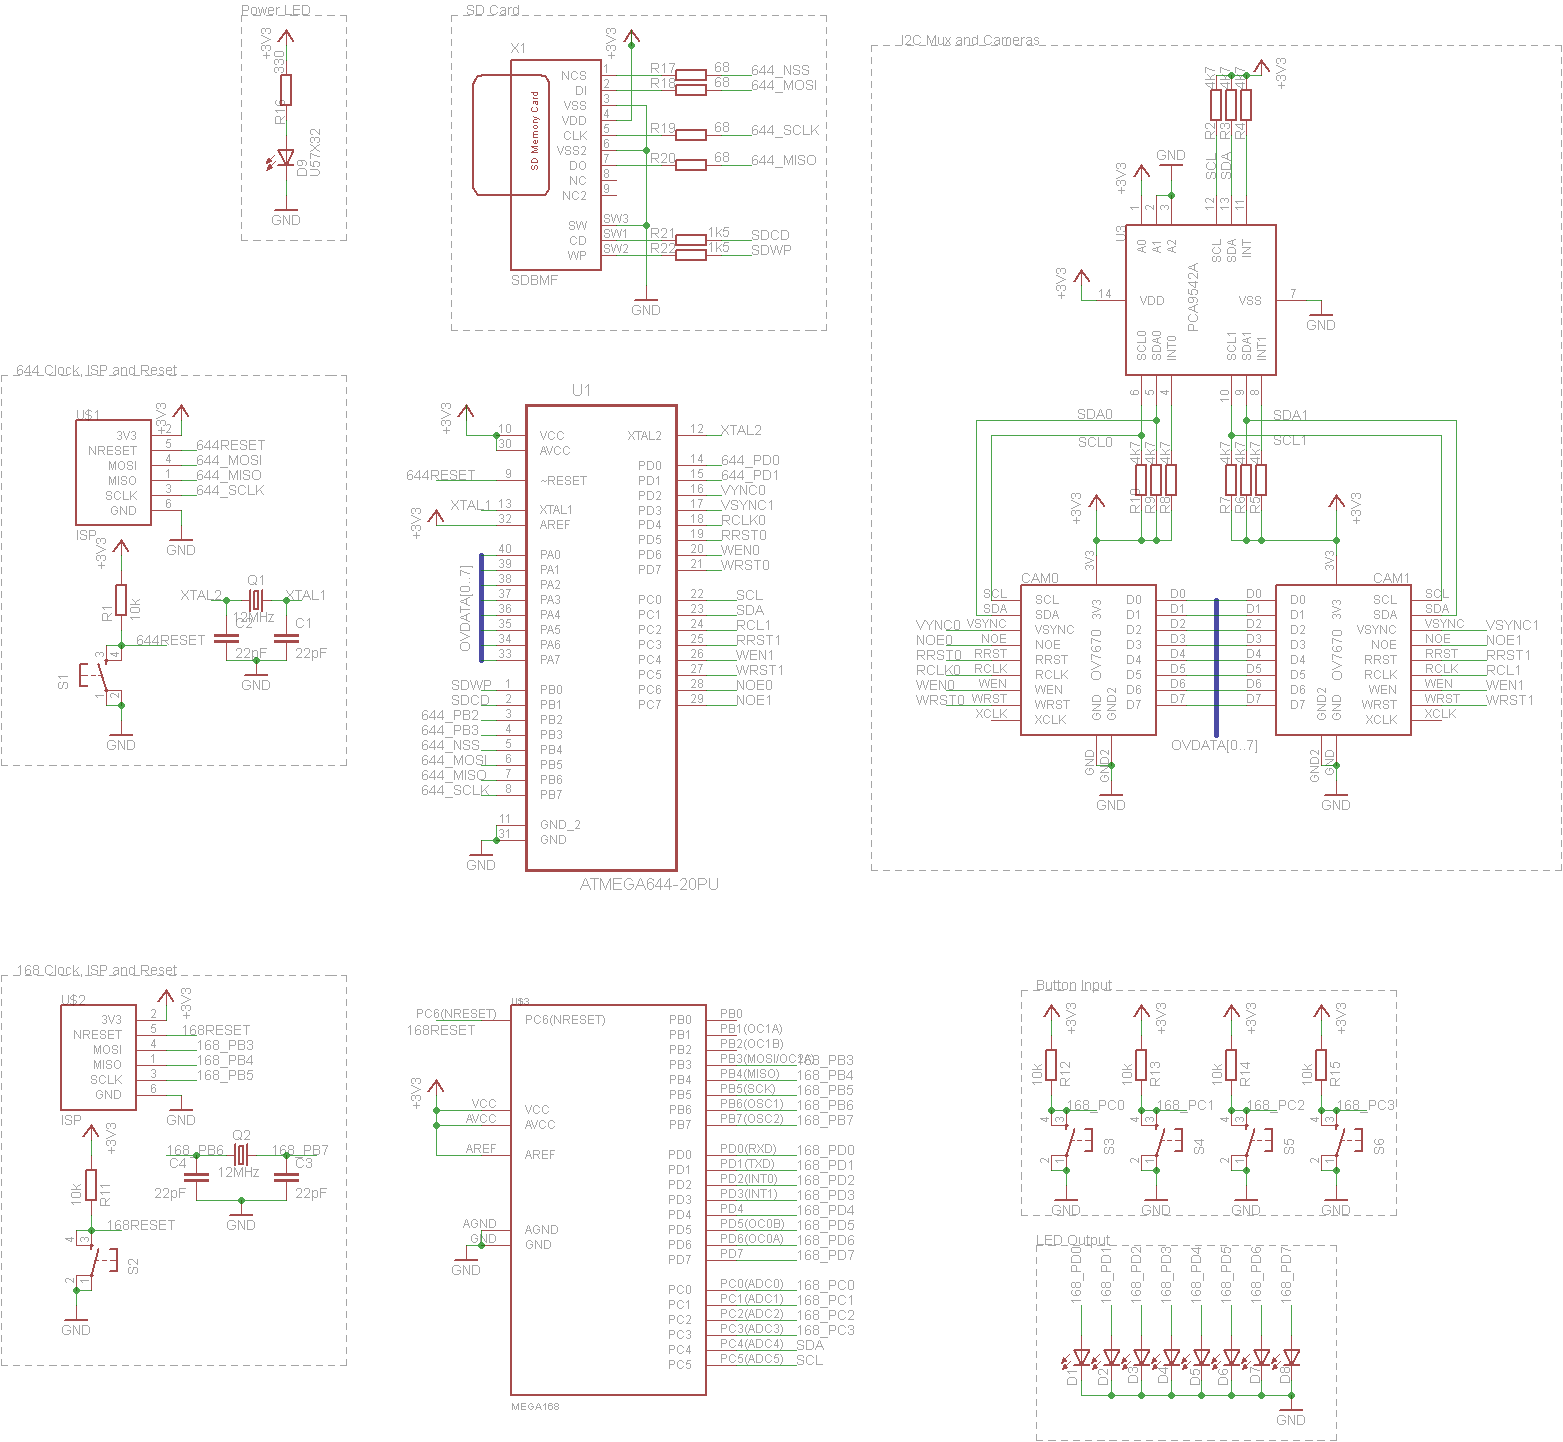
\includegraphics[angle = 90, width=\textwidth,height=\textheight,keepaspectratio]{Figures/IlMattoCamera_CircuitDiagram.png} 
\caption{The circuit diagram for Dual Cameras using the Il Matto Board}
\label{sch:DualCam_Schematic}

\end{figure}
\backmatter
\bibliographystyle{ecs}
%\bibliographystyle{unsrt}
\bibliography{ECS}
\end{document}
%% ----------------------------------------------------------------
